\documentclass{article}
\usepackage{graphicx} % Required for inserting images
\usepackage{amsmath}

\title{Séries temporais}
\author{Mariana Fernandes Rocha}
\date{September 2025}

\begin{document}


\begin{titlepage}
    \begin{center}

        \vspace{1cm}
        \begin{minipage}{0.45\textwidth}
            \centering
            
\includegraphics[width=1.2\textwidth]{images/logo_fgv.png}    
        \end{minipage}
        \vspace{2cm}

        \rule{1\textwidth}{0.4pt} \\ % Linha horizontal personalizada
        \vspace{0.3cm}
        {\Huge \textbf{Análise de Séries Temporais}} \\
        \vspace{0.2cm}
        \vspace{0.5cm}\\
        {\Large \textbf{A1 Séries Temporais}}\\
        \rule{1\textwidth}{0.4pt} % Linha horizontal personalizada


        \vspace{0.5cm}
        {\Large \textbf{FGV EMAp}} \\
        \vspace{2cm}
        
        

        
        
        % % Unidade e curso
        % {\Large \textbf{FGV EMAp}}\\[2cm]
        
        % Autores
        {\large 
            \textbf{Ana Júlia Amaro Pereira Rocha} \\ 
            \textbf{Henrique Borges Carvalho} \\
            \textbf{Maria Eduarda Mesquita Magalhães}\\
            \textbf{Mariana Fernandes Rocha} \\
            \textbf{Paula Eduarda de Lima}}\\[1.5cm]
        
        % Informações adicionais
        {\large 
            Ciência de Dados e Inteligência Artificial \\ 
            6º Período}\\[2cm]
        
         % Data
        \vfill
        {\large Rio de Janeiro, 2025}

        
    \end{center}
\end{titlepage}

\section{Discussão sobre métricas e métodos de avaliação}

Para previsões pontuais temos dois grupos de métricas e avaliação:
\begin{itemize}
    \item Métricas percentuais;
    \item Métricas escaladas;
\end{itemize}

Métricas percentuais são adequadas para cenários em que os valores devem ter uma ordem de grandeza clara e consistente, e mais importante assumir valores distantes de zero, devido a distorções que os erros sofrem quando $$y_t \to 0, \dfrac{e_t}{y_t} \to \infty$$

 Primeiramente, mais um terço dos dados assumem valores menores 1, o intervalo que mais sofre com a distorção. Outro ponto, o intervalo dos dados $[0.14 , 16.59]$ não representa uma escala de grandeza bem compreendida, e com esses argumentos concluímos que métricas percentuais não são convenietens para nossos dados

\begin{figure}[h]
    \centering
    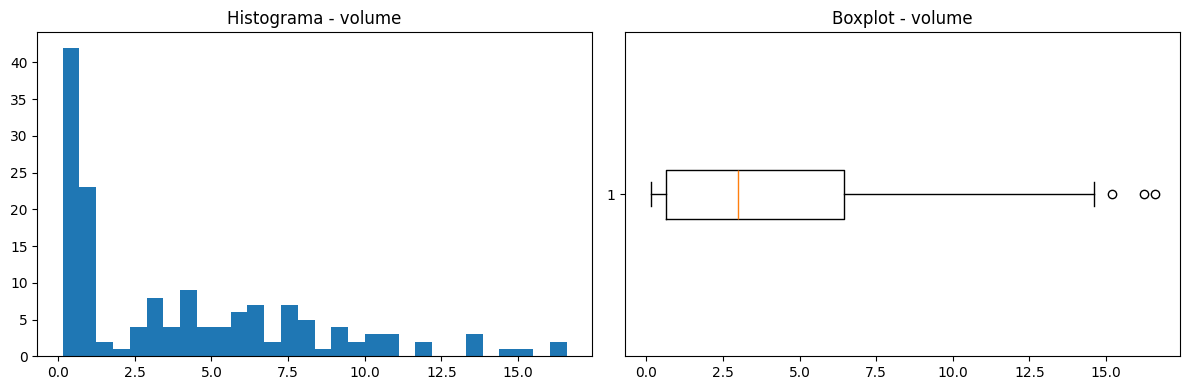
\includegraphics[width=0.75\linewidth]{images/histogram.png}
    \caption{Histograma e distribuição dos valores}
    % \label{fig:placeholder}
\end{figure}

Métricas escaladas não sofrem do mesmo problema, com a vantagem de conseguirmos comparar séries de 



\section{Discussão sobre a necessidade de transformação de variáveis}


\section{Discussão sobre a necessidade de decomposição entre tendência e sazonalidade}

\section{Análises de resíduos e ajuste dos modelos}
\section{Modelos baselines}

\section{Modelos de regressão linear múltipla}






\end{document}
